\titledquestion{Mathématiques du signal}

Considérons le signal suivant :
$$x(t) = 2\cos(3\pi t) + \sin(6\pi t).$$

\vskip2ex

\begin{parts}
    \part Quelle est la transformée de Fourier de $x(t)$ ? Identifiez les fréquences présentes dans le signal et dessinez le spectre $|X(f)|$.
    \begin{solutionbox}{18cm}
        Pour trouver la transformée de Fourier de $x(t)$, on utilise les formules classiques :
        
        \begin{align*}
            \cos(3\pi t) &= \frac{e^{i3\pi t} + e^{-i3\pi t}}{2}\\
            \sin(6\pi t) &= \frac{e^{i6\pi t} - e^{-i6\pi t}}{2i}
        \end{align*}
        
        Donc :
        \begin{align*}
            x(t) &= 2 \cdot \frac{e^{i3\pi t} + e^{-i3\pi t}}{2} + \frac{e^{i6\pi t} - e^{-i6\pi t}}{2i}\\
            &= e^{i3\pi t} + e^{-i3\pi t} + \frac{1}{2i}e^{i6\pi t} - \frac{1}{2i}e^{-i6\pi t}
        \end{align*}
        
        La transformée de Fourier est :
        $$X(f) = \delta(f - 1.5) + \delta(f + 1.5) + \frac{1}{2i}\delta(f - 3) - \frac{1}{2i}\delta(f + 3)$$
        
        où les fréquences sont $f_1 = 1.5$ Hz (de $\cos(3\pi t)$) et $f_2 = 3$ Hz (de $\sin(6\pi t)$).
        
        Le spectre d'amplitude $|X(f)|$ est :
        $$|X(f)| = \delta(f - 1.5) + \delta(f + 1.5) + \frac{1}{2}\delta(f - 3) + \frac{1}{2}\delta(f + 3)$$
        
        \begin{center}
            \begin{tikzpicture}
                \begin{axis}[
                    axis lines=middle,
                    xlabel={$f$ (Hz)},
                    ylabel={$|X(f)|$},
                    xmin=-4, xmax=4,
                    ymin=-0.2, ymax=1.5,
                    width=12cm,
                    height=6cm,
                    ytick={0, 0.5, 1},
                    xtick={-3, -1.5, 0, 1.5, 3},
                    xticklabels={$-3$, $-1.5$, $0$, $1.5$, $3$}
                ]
                    % Dirac delta à f = -3
                    \draw[thick, blue, ->] (axis cs:-3,0) -- (axis cs:-3,0.5);
                    \node[above] at (axis cs:-3,0.5) {$\frac{1}{2}$};
                    
                    % Dirac delta à f = -1.5
                    \draw[thick, blue, ->] (axis cs:-1.5,0) -- (axis cs:-1.5,1);
                    \node[above] at (axis cs:-1.5,1) {$1$};
                    
                    % Dirac delta à f = 1.5
                    \draw[thick, blue, ->] (axis cs:1.5,0) -- (axis cs:1.5,1);
                    \node[above] at (axis cs:1.5,1) {$1$};
                    
                    % Dirac delta à f = 3
                    \draw[thick, blue, ->] (axis cs:3,0) -- (axis cs:3,0.5);
                    \node[above] at (axis cs:3,0.5) {$\frac{1}{2}$};
                \end{axis}
            \end{tikzpicture}
        \end{center}
    \end{solutionbox}
    
    \part Dessinez le spectre $|X_s(f)|$ du signal échantillonné $x_s(t)$ pour des fréquences d'échantillonnage de $f_e = 5$ Hz et $f_e = 7$ Hz. Que constatez-vous ?
    \begin{solutionbox}{20.5cm}
        La fréquence maximale du signal est $f_{max} = 3$ Hz. La fréquence de Nyquist est donc $f_{max} = 3$ Hz, ce qui signifie qu'il faut échantillonner à $f_e > 6$ Hz pour éviter le repliement spectral.
        
        \textbf{Échantillonnage à $f_e = 5$ Hz :}
        
        Comme $f_e = 5$ Hz $< 6$ Hz, il y a repliement spectral. Le spectre se répète périodiquement tous les 5 Hz.
        La fréquence de Nyquist est $f_e/2 = 2.5$ Hz.
        
        \begin{itemize}
            \item La fréquence $f = 1.5$ Hz $< 2.5$ Hz, donc pas de repliement.
            \item La fréquence $f = 3$ Hz $> 2.5$ Hz, donc repliement : $3$ Hz se replie à $5 - 3 = 2$ Hz.
            \item Les fréquences négatives se replient également : $-1.5$ Hz se replie à $-1.5 + 5 = 3.5$ Hz, et $-3$ Hz se replie à $-3 + 5 = 2$ Hz.
        \end{itemize}
        
        Le spectre échantillonné contient des impulsions aux fréquences : $-3.5$, $-2$, $-1.5$, $1.5$, $2$, $3.5$ Hz (et leurs répétitions périodiques tous les 5 Hz).
        
        \begin{center}
            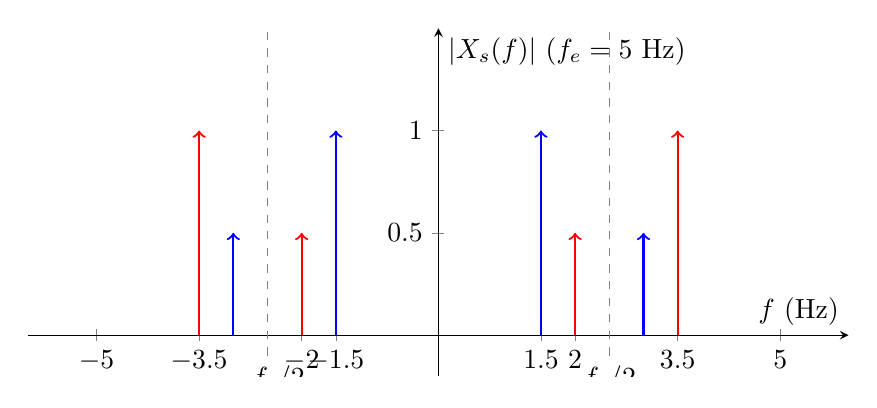
\begin{tikzpicture}
                \begin{axis}[
                    axis lines=middle,
                    xlabel={$f$ (Hz)},
                    ylabel={$|X_s(f)|$ ($f_e = 5$ Hz)},
                    xmin=-6, xmax=6,
                    ymin=-0.2, ymax=1.5,
                    width=12cm,
                    height=6cm,
                    ytick={0, 0.5, 1},
                    xtick={-5, -3.5, -2, -1.5, 0, 1.5, 2, 3.5, 5},
                    xticklabels={$-5$, $-3.5$, $-2$, $-1.5$, $0$, $1.5$, $2$, $3.5$, $5$}
                ]
                    % Répétitions périodiques (une période de chaque côté)
                    % Période -5 à 0
                    \draw[thick, blue, ->] (axis cs:-3,0) -- (axis cs:-3,0.5);
                    \draw[thick, red, ->] (axis cs:-3.5,0) -- (axis cs:-3.5,1);
                    \draw[thick, red, ->] (axis cs:-2,0) -- (axis cs:-2,0.5);
                    \draw[thick, blue, ->] (axis cs:-1.5,0) -- (axis cs:-1.5,1);
                    % Période 0 à 5
                    \draw[thick, blue, ->] (axis cs:1.5,0) -- (axis cs:1.5,1);
                    \draw[thick, red, ->] (axis cs:2,0) -- (axis cs:2,0.5);
                    \draw[thick, blue, ->] (axis cs:3,0) -- (axis cs:3,0.5);
                    \draw[thick, red, ->] (axis cs:3.5,0) -- (axis cs:3.5,1);
                    % Ligne pointillée pour f_e/2
                    \draw[dashed, gray] (axis cs:-2.5,-0.1) -- (axis cs:-2.5,1.5);
                    \draw[dashed, gray] (axis cs:2.5,-0.1) -- (axis cs:2.5,1.5);
                    \node[below] at (axis cs:-2.5,-0.1) {$-f_e/2$};
                    \node[below] at (axis cs:2.5,-0.1) {$f_e/2$};
                \end{axis}
            \end{tikzpicture}
        \end{center}
        
        \textbf{Échantillonnage à $f_e = 7$ Hz :}
        
        Comme $f_e = 7$ Hz $> 6$ Hz, il n'y a pas de repliement spectral. Le spectre se répète périodiquement tous les 7 Hz sans distorsion.
        
        \begin{center}
            \begin{tikzpicture}
                \begin{axis}[
                    axis lines=middle,
                    xlabel={$f$ (Hz)},
                    ylabel={$|X_s(f)|$ ($f_e = 7$ Hz)},
                    xmin=-7, xmax=7,
                    ymin=-0.2, ymax=1.5,
                    width=12cm,
                    height=6cm,
                    ytick={0, 0.5, 1},
                    xtick={-7, -3, -1.5, 0, 1.5, 3, 7},
                    xticklabels={$-7$, $-3$, $-1.5$, $0$, $1.5$, $3$, $7$}
                ]
                    % Période -7 à 0
                    \draw[thick, blue, ->] (axis cs:-3,0) -- (axis cs:-3,0.5);
                    \draw[thick, blue, ->] (axis cs:-1.5,0) -- (axis cs:-1.5,1);
                    % Période 0 à 7
                    \draw[thick, blue, ->] (axis cs:1.5,0) -- (axis cs:1.5,1);
                    \draw[thick, blue, ->] (axis cs:3,0) -- (axis cs:3,0.5);
                    % Ligne pointillée pour f_e/2
                    \draw[dashed, gray] (axis cs:-3.5,-0.1) -- (axis cs:-3.5,1.5);
                    \draw[dashed, gray] (axis cs:3.5,-0.1) -- (axis cs:3.5,1.5);
                    \node[below] at (axis cs:-3.5,-0.1) {$-f_e/2$};
                    \node[below] at (axis cs:3.5,-0.1) {$f_e/2$};
                \end{axis}
            \end{tikzpicture}
        \end{center}
        
        \textbf{Conclusion :} Avec $f_e = 5$ Hz, on observe un repliement spectral : la fréquence $3$ Hz se replie à $2$ Hz, créant de la distorsion. Avec $f_e = 7$ Hz, le spectre est préservé sans repliement, confirmant le théorème de Shannon-Nyquist.
    \end{solutionbox}
\end{parts}
